%
\chapter{Conceitos Fundamentais e Revisão Bibliográfica}
\label{chap:revisaobibliografica}
%\emph{Texto não obrigatório}

\section{Gasolina de Pirólise (\emph{PYGAS})} \label{sec:pygas}
A gasolina de pirólise (\emph{PYGAS - Pyrolysis Gasoline}) é um dos produtos
obtidos no processo de craqueamento a vapor quando da produção de olefinas na
indústria petroquímica. Tipicamente a gasolina de pirólise apresenta curva de
destilação entre 303K e 477K ou mais. Ela é um produto instável (térmica e
químicamente) devido à grande quantidade de compostos insaturados tais como:
monoolefinas, diolefinas conjugadas, estireno e outras espécies mais pesadas e
também reativas \cite{Cheng1986}.
\nomenclature[Z]{PYGAS}{Gasolina de pirólise}
 
A grande quantidade de de compostos insaturados (olefinas e aromáticos) contidos
na gasolina de pirólise lhe fazem um produto interessante, tanto pela
sua alta octanagem quanto pela sua quantidade de aromáticos. Contudo, a
instabilidade (formação de goma, cor) impede sua utilização comercial na forma como é produzida. Assim,
processos de refinamento específicos para essa corrente são necessários
\cite{Derrien1986}.

O esquema de processo a ser utilizado para refinar a gasolina de pirólise
depende do produto final desejado. Para a produção de uma corrente que
comporá a gasolina automotiva, atendendo requisitos tais como estabilidade e
corrosividade, é aplicado a hidrogenação seletiva de diolefinas, também
conhecido como primeiro estágio de hidrogenação. Já se o propósito for a
obtenção de aromáticos, segue-se à hidrogenação seletiva o segundo estágio
de hidrogenação (hidrogenação de olefinas e hidrodessulfurização)
\cite{Derrien1986}.

\section{Reatores de Leito Gotejante} \label{sec:reatorestbr}

\subsection{Definição} \label{sec:definicao}

Na literatura encontram-se vários autores que trataram das definições de
reatores catalíticos multifásicos de leito empacotado (PBR - \emph{Packed Bed
Reactors}).
\nomenclature[Z]{PBR}{Reator de leito empacotado}

Segundo \citeonline{Froment2011}, por reatores de leito empacotado multifásicos
entende-se as colunas que possuem recheios catalíticos, e que são destinadas a
promover reações entre compostos presentes em ambas as fases gasosa e líquida.

Assim como \citeonline{Froment2011}, \citeonline{Ancheyta2011} acrescenta à
definição de PBR uma distinção quanto ao regime de escoamento e direção de
escoamento das fases, sendo duas as formas: (i) em regime gotejante, onde a fase
gás é contínua e a fase líquida está distribuída, e a principal resistência a
transferência de massa está na fase gasosa; e (ii) em regime de borbulhamento,
com a fase gás distribuída e a fase líquida contínua, e a principal resistência
a transferência de massa localiza-se na fase líquida.

Os reatores de leito gotejante (TBR - \emph{Trickle Bed Reactor}) compreendem uma família de
PBRs nos quais as fases gasosa e líquida escoam através de um leito catalítico fixo, sendo eles assim classificados como reatores de leito fixo (FBR - \emph{Fixed Bed Reactors}). O TBR ainda possui as seguintes características, segundo \citeonline{Ancheyta2011}.
\nomenclature[Z]{TBR}{Reator de leito gotejante}
\nomenclature[Z]{FBR}{Reator de leito fixo}

\begin{itemize}
\item A fase líquida escoa em sentido descendente (na direção da gravidade),
fluindo sob a forma de filmes, filetes (\emph{rivulet}) e gotículas (e é daí
que vem o nome \textit{gotejante} (\emph{trickle}));
\item A fase gasosa pode escoar tanto ascendentemente (contracorrente à
fase líquida) quando descendentemente (cocorrente à fase líquida)
\end{itemize}

Os PBRs nos quais há escoamento ascendente tanto da fase gasosa quanto da
fase líquida opera em regime de borbulhamento, não este tipo de reator,
portanto, classificado entre os TBR \cite{Ancheyta2011}. Vale lembrar que

A configuração convencional dos TBRs está representada na
\autoref{fig:configuracoestbr}.

 \begin{figure}[htb]
 \centering 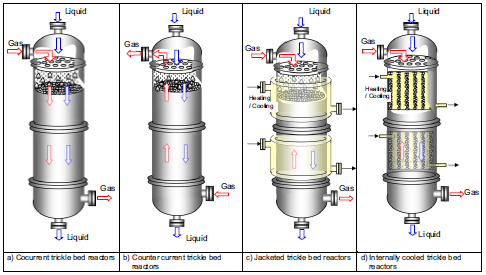
\includegraphics[scale=0.75]{images/Chap2/configuracoestbr.png}
 \caption{Regimes de escoamento em reatores de leito gotejante \cite{Gunjal2005}.}
 \label{fig:configuracoestbr}
 \end{figure}


\subsection {Regimes de Escoamento}
\label{sec:escoamento}

Um TBR pode ser visualizado como um leito de partículas de catalisador, no qual
o espaço intersticial entre elas formam complexos caminhos e distribuição de
poros. Ao fluir sobre as partículas de catalisador, gás e líquido podem
apresentar diferentes tipos de escoamento ou regimes. Esses regimes de
escoamento dependem da da densidade do leito, da velocidade de escoamento das
fases, do tamanho das partículas de catalisador, das dimensões do reator e das
propriedades físicas dos fluidos \cite{Ranade2011}.

A definição do tipo de escoamento, tanto na fase de projeto quanto na avaliação
de um reator existente, é muito importante pois vários parâmetros
hidrodinâmicos e de transporte são influenciados pelo regime de escoamento. Este
últimos influenciam tanto no dimensionamento dos TBRs quanto nos
equipamentos atrelados a eles, tais como bombas e compressores
\cite{Ranade2011}.

Segundo \apudonline{Ramachandran1983}{Ranade2011}, quatro
diferentes regimes de escoamento foram identificados em TBRs:

\begin{itemize}
	\item Gotejamento (\emph{Trickle flow regime)},
	\item de pulso (\emph{Pulse flow regime)},
	\item Spray (\emph{Spray flow regime)}, e
	\item Borbulhamento (\emph{Buble flow regime)}
\end{itemize}

Esses regimes de escoamento estão ilustrados na \autoref{fig:regimeescoamento}.

 \begin{figure}[htb]
 \centering 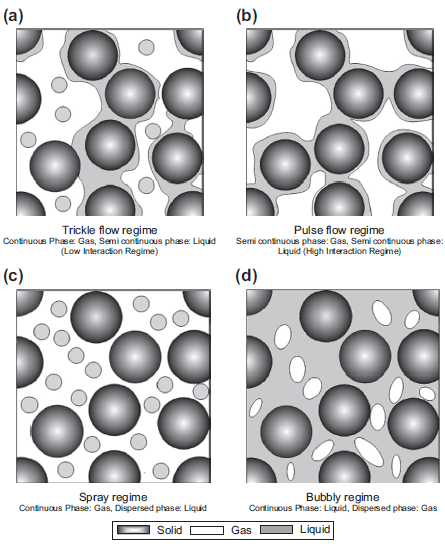
\includegraphics[scale=0.75]{images/Chap2/regimeescoamento.png}
 \caption{Regimes de escoamento em reatores de leito gotejante \cite{Gunjal2005}.}
 \label{fig:regimeescoamento}
 \end{figure}

O escoamento em regime gotejante ocorre em baixo fluxo de líquido e moderado
fluxo de gás. Como já foi dito, o líquido escoa em forma de filmes ou filetes
sobre as partículas do catalisador. Nesse regime de escoamento, a fase contínua
é a gasosa e a fase líquida escoa dispersa. Esse tipo de escoamento também é
chamado de regime de baixa interação \cite{Saroha1996}.

Em fluxo moderado de líquido e gás ocorre o escoamento em regime de pulso,
caracterizado pelo escoamento semicontínuo de ambas as fases. Ante o regime
por gotejamento, o regime de pulso apresenta maior interação entre as fases.
Todavia, esse processo faz com que regiões ricas em gás se alternem com regiões
ricas em líquido \cite{Saroha1996}.

Os outros dois regimes de escoamento encontrados em TBRs são: borbulhamento e
tipo spray. No primeiro, a fase contínua é a líquida, enquanto que a fase gasosa
escoa dispersa; no segundo, a fase contínua é a gasosa, e a fase líquida é
dispersa. Ambos os casos são classificados como regimes de alta interação entre
as duas fases \cite{Saroha1996}.

Os reatores industriais operam com frequência na próximos a transição entre os
regimes gotejante e pulsado. Isso proporciona melhores taxas de transferência de
massa, utilização do catalisador e aumenta a capacidade produtiva
\cite{Ancheyta2011}.

\subsection{Parâmetros Hidrodinâmicos}
\label{sec:parametroshidrodinamicos}

Por natureza, os TBRs possuem uma comlexidade fenomenológica ímpar quando se
trata de seu comportamento hidrodinâmico. Supera em complexidade tanto os FBRs,
onde somente há apenas uma fase escoando pelo leito catalítico, quanto colunas
empacotadas onde não há transferência de massa. 

A compreensão e a previsão, ainda que imprecisamente, dos parâmetros
hidrodinâmicos dos TBRs são as chaves para o projeto e análise desse tipo de
reator. Os parâmetros que serão discorridos a seguir são:

\begin{itemize}
  \item Perda de carga
  \item Retenção de líquido
  \item Molhamento das partícutas de catalisador
  \item Coeficientes de transferência de massa
  \item Dispersões axial e radial de massa
%  \item Transferência de calor em TBRs
\end{itemize}

\subsubsection{Perda de Carga}
\label{sec:perdadecarga}

A capacidade de estimar a perda de carga em TBRs na fase de projeto é de suma
importância. Ela definirá a capacidade de um dos equipamentos mais custosos do
sistema, o compressor que fará a recirculação da fase gasosa. A perda de carga
também é um importante parâmetro a ser acompanhando pelos engenheiros quando o
TBR está em operação; evoluções abruptas na perda de carga nos leitos
catalíticos normalmente é um indicador de um problema sério de
escoamento.

A perda de carga bifásica ao longo do reator está relacionada com: (i) a
geometria do reator (diâmetro, tamanho e forma do catalisador e geometria dos
internos, tais como prato distribuidor); parâmetros operacionais tais como vazão
de gás e líquido (regime de escoamento); e propriedades das fases (densidade,
viscosidade, tensão superficial etc.). Temperatura e pressão de operação afetam
indireamente a perda de carga através das propriedades do fluido
\cite{Ranade2011}.

Normalmente as equações de perda de carga são definidas em termos de perda de
carga específica $\Delta P/l$, que é definida como a variação da pressão interna
por unidade de comprimentos do reator. Em reatores cujo regime é de baixa
interação (regime gotejante de escoamento), a perda de carga tende a ser
pequena. Para regimes de alta interação, a perda de carga pode chegar a alguns
atmosferas por metro \cite{Benkrid1997}.

\nomenclature[G]{$\Delta P/l$}{Perda de carga específica \nomunit{kPa/m}} 

Segundo \citeonline{Holub1993}, os modelos hidrodinâmicos podem ser
classificados em duas categorias. A primeira categoria lança mão do empirismo
baseado em análise dimensional para produzir correlações de perda de carga e
retenção de líquido. A segunda categoria utiliza equações tipo Ergun
\apud{Ergun1952}{Holub1993}, modificando parâmetros para escoamento bifásico.
Essa abordagem é aplicada especialmente para regimes de escoamento de baixa
interação.

\citeonline{Holub1993}, por exemplo, desenvolveram uma correlação para perda
de carga para TBRs operando em regimes de baixa interação. Já
\citeonline{Benkrid1997} utilizaram dados experimentais  da literatura para propor modelos
simples de perda de carga em TBRs que operam em regimes de alta
interação. Ambos autores citados neste parágrafo também desenvolveram
correlações para retenção de líquido.

Diferentemente de muitos autores, que propuseram equações utilizando dados
experimentais coletados em pressões atmosféricas, \citeonline{Larachi1991}
construiu correlações tanto para perda de carga quanto para retenção de líquido
, em pressões de até 8.1 MPa.

\subsubsection{Retenção de Líquido}
\label{sec:retencaodeliquido}

A retenção de líquido (\emph{liquid holdup})em um leito de TBR  pode ser
expressada de duas maneiras: (i) retenção total ($\epsilon_L$), definida
como o volume de líquido por unidade de volume de leito e (ii) saturação de líquido
($\beta_L$), definida como o volume de líquido por unidade de volume vazio
(ao invés de volume total de leito). 

A retenção de líquido é composta de duas partes: estática ($\epsilon_{Ls}$) e
dinâmica ($\epsilon_{Ld}$). Por renteção de líquido estática entende-se a porção
de líquido que permanece na superfície das partículas de catalisador após o
leito ser drenado. A fração removida de líquido é definida como retenção
dinâmica \cite{Ranade2011}. Alguns autores utilizam como referência a saturação
de líquido estática ($\beta_{Ls}$) e saturação de líquido dinâmica ($\beta_{Ld}$).

Há algumas ténicas para determinação da retenção de líquido em TBRs. De acordo
com \cite{Benkrid1997}, a técnica mais comum é a da drenagem, já mencionada.
Essa técnica consiste em cessar simultaneamente a alimentação de gás e líquido
no reator (topo), coletando o líquido na saída (fundo). O volume de líquido
drenado significará diretamente $\epsilon_{Ld}$. Outra técnica é consiste em
determinar a massa do reator enquanto seco e em operação, quando gás e líquido
estarão escoando pelo leito catalítico. Esse método levará diretamente a
determinação de $\beta_L$. \cite{Larachi1991} utiliza a distribuição do tempo de
residência para chegar a $\beta_L$.

Vários fatores em TBRs são dependentes da retenção de líquido, tais como fator
de molhabilidade e coefientes de transferência de massa e calor. A retenção de
líquido também determina o tempo de residência de líquido dentro do reator e,
portanto, a conversão dos reagentes \cite{Ranade2011}.

\nomenclature[G]{$\epsilon_{L}$}{Retenção total de líquido}
\nomenclature[G]{$\epsilon_{Ls}$}{Retenção estática de líquido}
\nomenclature[G]{$\epsilon_{Ld}$}{Retenção dinâmica de líquido}
\nomenclature[G]{$\beta_L$}{Saturação de líquido}
\nomenclature[G]{$\beta_{Ls}$}{Saturação de líquido estática}
\nomenclature[G]{$\beta_{Ld}$}{Saturação de líquido dinâmica}

\subsubsection{Molhamento das Partículas de Catalisador}
\label{sec:molhamento}

Dentre os difersos tipos de reatores multifásicos, o molhamento das partículas
de catalisador é um fenômeno exclusivo em TBR. Levando-se em conta que, em um
TBR, a fase líquida escoa de forma não uniforme, a determinação do molhamento do
catalisador é uma tarefa bastante difícil \cite{Ranade2011}

Na literatura são definidos dois tipos de molhamento. \citeonline{Colombo1976}
os descreve assim:

\begin{itemize}
	\item Molhamento interno ou enchimento de poro: é o volume de líquido dentro
	dos poros do catalisador. Como as partículas de catalisador são quase sempre
	porosas, o molhamento interno é considerado total devido ao efeito de
	capilaridade.
	\item Molhamento externo: é a área externa à partícula de catalisador
	efetivamente em contato com o líquido que escoa. Praticamente toda a
	transferência de massa entre o líquido presente nos poros do catalisador e o
	líquido que escoa por sobre as partículas ocorre nessa área.
\end{itemize}

Isto posto, a \emph{eficiência de molhamento} ($\eta_{CE}$) deriva da definição
de molhamento externo. Em outras palabras, ela é definida como sendo a
porcentagem da área superficial externa do catalisador que está efetivamente em
contato com o líquido que escoa \cite{Schwartz1976}.

De uma forma geral, a medição da eficiência de molhamento pode ser direta e
indireta. Entre os métodos diretos estão técnicas fotográficas, método de
injeção de corante, imagem de ressonância magnética, entre outros
\apud{Sederman2001}{Ranade2011}. Já os métodos indiretos são aplicáveis a
unidades industriais além de possuirem melhor custo-benefício \cite{Ranade2011}.
\citeonline{Colombo1976} e \citeonline{Schwartz1976}, por exemplo, utilizaram
métodos baseados tanto em taxa de reação quanto em transferência de massa para
determinar a eficiência de molhamento.

\nomenclature[G]{$\eta_{CE}$}{Eficiência de molhamento}

\subsubsection{Coeficientes de Transferência de Massa}
\label{sec:coeficientes}

Em reatores com escoamento gotejante não há um mecanismo severo de mistura como
em outros tipos de escoamento (tanques de mistura ou regimes de alta interação).
Logo, as taxas de transferência de massa são menores em TBRs do que em outros
reatores, podendo limitar a taxa das reações. Os três tipos de taxas de
transferência de massa relevantes nos TBRs são: gás-líquido, líquido-sólido e
gás-sólido \cite{Ranade2011}.

A ocorrências desses tipos de transferência de massa dependerá da eficiência de
molhamento e da retenção de líquido. Em reatores com eficiência de molhamento
próxima a totalidade, por exemplo, desconsidera-se a transferência de massa
gás-sólido.

\subsubsection{Dispersões Axial e Radial de Massa}
\label{sec:dispersoes}

As dispersões axial e radial são dois fenômenos que ocorrem em TBRs,
desviando-os da idealidade de escoamento contida no conceito de PFR (PFR -
\emph{Plug-flow Reactor}).

\nomenclature[Z]{PFR}{Reator de escoamento empistonado}

A dispersão radial está diretamente ligada a distribuição de líquido na entrada
do reator. Esse efeito possui uma quantidade pequena de estudos na literatura.
Isso acontece porque, em reatores industriais, a instalação de distribuidores de
carga na entrada dos TBR (topo) promove uma distribuição radial de massa
uniforme. A razão entre o diâmetro do reator e diâmetro da partícula de
catalisador ($D_R/d_p$) tem se mostrado influente na distribuição radial de
massa \cite{Saroha1998}. \citeonline{Al-Dahhan1994}, por exemplo, sugerem que,
mesmo para reatores em alta pressão, um valor de $D_R/d_p > 20$ minimiza a má
distribuição de líquido.

Diferente do que ocorre com a dispersão radial, a dispersão axial é um fenômeno
amplamente estudado, com várias referências na literatura. Esse fenômeno está
ligado a retromistura de líquido dentro do leito catalítico e está relacionado
com a razão entre o comprimento do reator e diâmetro da partícula de catalisador
($L_R/d_p$) \cite{Ancheyta2011}.

\nomenclature{$D_{R}$}{Diâmetro do reator \nomunit{m}}
\nomenclature{$L_{R}$}{Comprimento do reator \nomunit{m}}
\nomenclature{$D_{R}$}{Diâmetro da partícula de catalisador \nomunit{m}}

Alguns fatores que contribuem na distribuição de líquido e na retromistura são:
capilaridade, zonas-morta, molhamento parcial e caminhos preferenciais
\cite{Ranade2011}.

\subsection{Reações Químicas em TBR} \label{sec:reacoes}
 
Os TBRs diferem dos reatores monofásicos de leito fixo exatamente pela presença
de uma terceira fase. Em outras palavras, uma camada a mais de resistência a
transferência de massa, tanto de reagentes quanto de produtos, é adicionada
ao sistema. 

Sendo assim, segundo\ldots, itens sequenciais (figura?)

Nos FBRs, a reação química intrínseca é aquela que considera os
seguintes fenômenos:
\begin{enumerate}
\item Adsorção dos reagentes na superfície catalítica; 
\item Reação química propriamente dita entre os reagentes; e
\item Desorção
\end{enumerate}  

modelos cinéticos simplificados que não descrevem o comportamento real na
superfície do catalisador.

%Daqui para baixo é a dissertação da Paula, mantida por questões de praticidade

O equilíbrio termodinâmico é alcançado quando são satisfeitas as condições de equilíbrio químico, térmico e
mecânico entre as fases:
\begin{equation}
\begin{array}{c}
% \phi_{liq_i} \cdot x_{out} = \phi_{vap_i} \cdot y_{out} \\
\hat{f}^L_i = \hat{f}^V_i \qquad (i = 1,2,...,c) \\
T^L = T^V \\
P^L = P^V \\
\end{array}
\end{equation}
onde, $\hat{f}_i$ é a fugacidade da espécie ou componente $i$ em solução, o superscrito
$L$ é utilizado para o líquido e $V$ para o vapor, $T$ e $P$ são a temperatura
e a pressão, respectivamente.


A igualdade de fugacidades, como apresentada acima, frequentemente é
representada utilizando coeficientes de fugacidade.
O coeficiente de fugacidade de um componente $i$, em uma solução gasosa, é
definido como:
\begin{equation}
\hat{\phi}^V_i \equiv \dfrac{\hat{f}^V_i}{Py_i} \qquad (i = 1,2,...,c) \\
\label{eq:phidefinition}
\end{equation}

\nomenclature[G]{$\hat{\phi}^L_i$}{Coeficiente de fugacidade da espécie $i$ em
solução líquida}
% \nomenclature{$\phi^L_i$}{Coeficiente de fugacidade da espécie $i$ pura, na fase
% % líquida}
\nomenclature[G]{$\hat{\phi}^V_i$}{Coeficiente de fugacidade da espécie $i$ em
solução gasosa}

Embora mais usual para gases, o coeficiente de fugacidade também
está definido para líquidos, pela \autoref{eq:phidefinitionL}, gerando o coeficiente $\hat{\phi}^L_i$.
\begin{equation}
\hat{\phi}^L_i \equiv \dfrac{\hat{f}^L_i}{Px_i} \qquad (i = 1,2,...,c) \\
\label{eq:phidefinitionL}
\end{equation}
Isto permite escrever a igualdade de fugacidades da seguinte forma:
\begin{equation}
\hat{\phi}^L_i x_i = \hat{\phi}^V_i y_i \qquad (i = 1,2,...,c) \\
\label{eq:phiequality}
\end{equation}
É importante notar que, embora a \autoref{eq:phiequality} envolva o
coeficiente de fugacidade, ela é geral o suficiente para tratar os casos onde
modelos de atividade são utilizados.
Isto pode ser verificado utilizando-se a definição do coeficiente de atividade
de um componente $i$ em uma solução líquida, como desvio em relação a regra de Lewis-Randall:
\begin{equation}
\gamma_i \equiv \dfrac{\hat{f}^L_i}{x_if^L_i} \qquad (i = 1,2,...,c) \\
\label{eq:gammadefinition}
\end{equation}
onde, $f^L_i$ é a fugacidade da espécie $i$ pura.

Das relações acima, é fácil demonstrar que $\hat{\phi}^L_i = \gamma_i \phi^L_i$,
com $\phi^L_i$ sendo o coeficiente de fugacidade do líquido $i$ puro, ou seja, $f^L_i = \phi^L_i P$. Assim,
para determinar o valor de $\hat{\phi}^L_i$,
basta associar um modelo de atividade (cálculo de $\gamma_i$) com uma equação de
estado (cálculo de $\phi^L_i$).
No pacote termodinâmico utilizado neste trabalho, esta é a forma de determinação
dos coeficientes de fugacidade quando modelos de atividade são utilizados.
Outra opção usual é aproximar $\phi^L_i$ como sendo simplesmente $P^{sat}_i/P$, onde
$P^{sat}_i$ é a pressão de vapor da espécie $i$ na temperatura de $T$, podendo-se ainda
fazer a correção de Poyting quando $P$ está distante de $P^{sat}_i$.

No caso de gases dissolvidos, pode-se utilizar a constante de Henry, $H_i$, associada ao coeficiente de
atividade à diluição infinita, $\gamma_{i,\infty}$, chegando-se na relação:
\begin{equation}
\hat{\phi}^L_i = \dfrac{\gamma_i H_i}{\gamma_{i,\infty} P} \qquad (i = 1,2,...,c) \\
\label{eq:gammadefinitionHenry}
\end{equation}

Neste caso, basta calcular $\phi^L_i = H_i / \gamma_{i,\infty} P$ e usar a mesma relação
$\hat{\phi}^L_i = \gamma_i \phi^L_i$.

O modelo desenvolvido neste trabalho, apresentado no \autoref{chap:moddesenvolvidos}, é baseado na condição de equilíbrio
termodinâmico.
Uma vez que o pacote de cálculo de propriedades utilizado neste trabalho
fornece os coeficientes de fugacidade independentemente do modelo termodinâmico
em uso, neste trabalho a forma apresentada na \autoref{eq:phiequality} é
preferida.

Geralmente, um estágio de separação de uma coluna de destilação é modelado com a hipótose de equilíbrio  termodinâmico
entre o vapor e o líquido existentes, mas na realidade, este equilíbrio não é alcançado. A primeira tentativa de corrigir
esta não-idealidade, ou não-equilíbrio, foi com a introdução de uma eficiência de estágio.
A eficiência de Murphree, que é um modelo de
eficiência muito utilizado, mede com que grau o equilíbrio termodinâmico é alcançado e é utilizada com certo sucesso em
sistemas binários e em estado estacionário. Porém, segundo \citeonline{Koeijer:2004}, não apresenta bons resultados
em simulações dinâmicas multicomponente.

Para explicar este desvio da idealidade no equilíbrio entre as fases, surgiu a
modelagem baseada em taxas de transferência, os chamados modelos de não-equilíbrio. De acordo com
essa corrente, a destilação é modelada por taxas de transferência que são
impulsionadas pela distância do equilíbrio e não mais pelo equilíbrio entre as
fases presentes. Nos primeiros trabalhos, as taxas de transferência foram modeladas
utilizando as equações de Maxwell-Stephan, o que acabou batizando o método
com o mesmo nome.

Assim, o método de Maxwell-Stephan se baseia na existência de um filme líquido e um filme de vapor com gradientes de
temperatura e concentração. Estes filmes entram em contato através de uma interface, onde é alcançada a condição de
equilíbrio termodinâmico entre as fases \cite{Koeijer:2004}.
% Esta estrutura pode ser vista na
% \autoref{fig:interfaceesquema}.
%  \begin{figure}[htb]
%  \centering \includegraphics[scale=0.9]{images/Chap2/interfaceesquema.png}
%  \caption{Interface entre as fases líquida e vapor considerada no método de Maxwell-Stephan \cite{Koeijer:2004}}.
%  \label{fig:interfaceesquema}
%  \end{figure}

A representação esquemática global de um estágio, onde não há equilíbrio termodinâmico, pode ser vista na
\autoref{fig:nonequilibriumstage}.
 \begin{figure}[htb]
 \centering \includegraphics[scale=0.6]{images/Chap2/nonequilibriumstage.png}
 \caption{Diagrama esquemático de um estágio sem consideração de equilíbrio termodinâmico \cite{Kooijman:1995a}.}
 \label{fig:nonequilibriumstage}
 \end{figure}
A linha vertical ondulada no meio do diagrama representa a interface entre as duas fases, que podem ser tanto líquido e
vapor (no caso de um estágio de destilação) como duas fases líquidas (no caso de
um processo de extração). Estas duas fases trocam massa e energia através das
taxas $N$ e $E$, respectivamente. O força motriz destas taxas é justamente a
consideração de não-equilíbrio entre as fases.

Geralmente, o modelo de um estágio real, ou seja, sem a condição de equilíbrio, é composto por três partes. A primeira,
com as equações de balanço de massa e energia para a fase líquida, a segunda com as equações de balanço da fase vapor,
e a terceira parte, unindo as anteriores, com as equações da interface referentes às taxas de transferência de massa
e energia e a relação de equilíbrio.

Na transferência de massa, as taxas molares de líquido e vapor contam com uma contribuição difusiva e uma convectiva,
conforme a \autoref{eq:fluxomolvap} e \ref{eq:fluxomolliq}. %\autoref{eq:equilfluxomol}, 
\begin{equation}
N^V_{ij} - N^L_{ij}= 0
\label{eq:equilfluxomol}
\end{equation}
\begin{equation}
N^V_{ij} = J^V_{ij}a_j^I + y_{ij}N_{tj}
\label{eq:fluxomolvap}
\end{equation}
\begin{equation}
N^L_{ij} = J^L_{ij}a_j^I + x_{ij}N_{tj}
\label{eq:fluxomolliq}
\end{equation}
onde $a^I_j$ é a área interfacial total no estágio $j$ e $N_{tj}$ é a taxa de
transferência de massa total no estágio $j$ com $N_{tj} =
\displaystyle\sum_{i=1}^c N_{ij}$

\nomenclature{$N^V_{ij}$}{Taxa de transferência molar do componente $i$ na fase vapor, no estágio $j$ \nomunit{mol/s}}
\nomenclature{$N^L_{ij}$}{Taxa de transferência molar do componente $i$ na fase líquida, no estágio $j$ \nomunit{mol/s}}
\nomenclature{$J^V_{ij}$}{Fluxo molar difusivo do componente $i$ no vapor, no estágio $j$ \nomunit{mol/(m^2\ s)}}
\nomenclature{$J^L_{ij}$}{Fluxo molar difusivo do componente $i$ no líquido, no estágio $j$ \nomunit{mol/(m^2\ s)}}
\nomenclature{$y_{ij}$}{Fração molar no vapor do componente $i$ no estágio $j$}
\nomenclature{$x_{ij}$}{Fração molar no líquido do componente $i$ no estágio $j$}
\nomenclature{$a^I_j$}{Área interfacial total no estágio $j$ \nomunit{m^2}}
\nomenclature{$N_{tj}$}{Taxa de transferência de massa total no estágio $j$ \nomunit{mol/s}}
\nomenclature{$C_t^V$}{Concentração molar total da fase vapor \nomunit{mol/m^3}}
\nomenclature{$C_t^L$}{Concentração molar total da fase líquida\nomunit{mol/m^3}}
O fluxo difusivo $J$, na forma matricial, é dado por:
\begin{equation}
\left( J^V\right)  = C_t^V \left[ k^V\right] \left( \overline{y^V-y^I}\right) 
\label{eq:diffusionvap}
\end{equation}
\begin{equation}
\left( J^L\right)  = C_t^L \left[ k^L\right] \left( \overline{x^I-x^L}\right) 
\label{eq:diffusionliq}
\end{equation}
onde $C_t^V$ é a concentração molar total da fase vapor, $C_t^L$ é a
concentração molar total da fase líquida, $k^V$ e $k^L$ são os coeficientes de transferência de massa e
$\left( \overline{y^V-y^I}\right)$ e $\left( \overline{x^I-x^L}\right)$ são as médias das diferenças das frações
molares entre a interface e o seio da fase vapor e líquida, respectivamente.
Para o cálculo dessas diferenças, existem inúmeras teorias e correlações. Estes
cálculos geralmente dependem da geometria do prato e das condições hidráulicas do mesmo. No trabalho de
\citeonline{Hongyan:2002}, é estudado o efeito dos gradientes de concentração no prato para o cálculo da eficiência e dos
coeficientes de transferência de massa, assim como o efeito do arraste de líquido sobre estes mesmos parâmetros. Ainda
nessa linha de pesquisa, \citeonline{Kooijman:1995a} reservou um capítulo inteiro da sua tese para mostrar os
diversos modelos de dispersão existentes e novas correlações, propostas pelo autor.

\nomenclature{$C$}{Concentração molar \nomunit{mol/m^3}}
\nomenclature{$k^L$}{Coeficiente binário de transferência de massa na fase líquida \nomunit{m/s}}
\nomenclature{$k^V$}{Coeficiente binário de transferência de massa na fase vapor \nomunit{m/s}}

% A matriz dos coeficientes de transferência de massa é calculada da seguinte maneira:
% \begin{equation}
% \left[ k^P\right]  = \left[ R^P\right]^{-1} \left[ \Gamma^P\right] 
% \label{eq:matrizcoefmass}
% \end{equation}
% onde $\left[ \Gamma^P\right]$ é chamada de matriz de fatores termodinâmicos da fase P e $\left[ R^P\right]$
% à matriz das resistências à transferência de massa. Os efeitos termodinâmicos têm uma grande importância
% nesse cálculo, pois a força
% motriz fundamental da transferência de massa é o potencial químico e não o gradiente de fração molar ou de concentração.
% A matriz $\left[ \Gamma^P\right]$ deve ser calculada com modelos termodinâmicos apropriados dependendo se são utilizadas
% equações de estado ou modelos de atividade. A matriz $\left[ R^P\right]$
% leva em consideração os coeficientes binários de transferência de massa, a forma do equipamento, parâmetros operacionais
% e propriedades físicas dos componentes envolvidos. Podem ser utilizadas as equações de Maxwell-Stephan para o cálculo da
% matriz $\left[ R^P\right]$. Para um maior detalhamento destes cálculos, ver
% \citeonline{Kooijman:1995a}.

Assim como para a massa, a taxa de transferência de energia na interface é escrita:
\begin{equation}
E^V_j -  E^L_j = 0
\label{eq:balancofluxoenergia}
\end{equation}
com as taxas de transferência de energia (calor) de ambas as fases definidas por:
\begin{equation}
E^V_j = a_j^I h^V \left( T^V - T^I\right) + \sum^c_{i=1} N^V_{ij}
\overline{H}^V_{ij}
\label{eq:taxaevj}
\end{equation}
\begin{equation}
E^L_j = a_j^I h^L \left( T^I - T^L\right) + \sum^c_{i=1} N^L_{ij}
\overline{H}^L_{ij}
\label{eq:taxaelj}
\end{equation}
onde $h^V$ e $h^L$ são os coeficientes convectivos de transferência de calor na fase vapor e na fase líquida,
$T^V$, $T^I$ e $T^L$ são as
temperaturas do vapor, interface e líquido e $\overline{H}_{ij}$ é a entalpia parcial molar do componente $i$ no estágio $j$.

Além das transferências de massa e energia, é adotada a condição de equilíbrio entre as fases na interface.
Vale ressaltar que o equilíbrio
termodinâmico de fases é considerado apenas na interface.

Uma grande desvantagem do modelo de não-equilíbrio é que o cálculo das taxas de
transferência requer o fornecimento de uma matriz de coeficientes de
transferência de massa, a qual necessita de dados experimentais. Infelizmente, esse
tipo de dado não está disponível em abundância na literatura, dificultando a utilização dessa modelagem.
Outro aspecto negativo é a necessidade do cálculo de propriedades de
misturas adicionais, quando comparado ao modelo de equilíbrio.
Estas propriedades adicionais são basicamente a tensão superficial,
viscosidade, condutividade térmica, além dos coeficientes de transferência de
massa.

Apesar das dificuldades, os modelos de não-equilíbrio tendem a representar a realidade de uma forma mais fidedigna que os
modelos de equilíbrio, conforme é relatado no trabalho de \citeonline{Biardi:1989} e de \citeonline{Kooijman:1995}. Por isso,
são mais utilizados para o projeto de novas unidades.

\section{Modelagem de Reatores de Leito Gotejante} \label{sec:modred}
Um modelo rigoroso típico de um prato de uma coluna de destilação consiste em equações que descrevem as
concentrações das espécies, vazões de líquido e vapor, temperatura, queda de pressão e relações de
equilíbrio (ou não) entre as
fases líquida e vapor. Considerando as grandes dimensões da maioria das colunas de destilação industriais, geralmente
com mais de 50 pratos, uma simulação rigorosa do comportamento dinâmico requer a resolução de um sistema de milhares
de equações. Este procedimento de resolução pode levar um considerável tempo computacional. Nestes casos, um modelo
reduzido pode ser necessário \cite{Musch:1993}. Além disso, muitas vezes o sistema
gerado apresenta um índice diferencial elevado. O índice diferencial é utilizado como uma medida da dificuldade de
solução numérica de sistemas algébrico-diferenciais. Sistemas com índice diferencial igual a 0 são, na verdade,
sistemas de equações diferenciais ordinárias. Sistemas com índice maior que 1 são conhecidos como sistemas de índice
elevado e não podem ser tratados diretamente por códigos integradores convencionais \cite{Brennan:1989}.

Foi durante a década de 80 que os principais trabalhos a cerca da redução de modelos foram publicados. Naquela época, os
métodos de solução dos sistemas de equações gerados pela modelagem dos processos de separação eram muito limitados. Não
havia integradores de sistemas de equações algébrico-diferenciais (\emph{Differential-Algebraic Equations} - DAE), apenas
integradores para sistemas ODE (\emph{Ordinary Differential Equations}). A solução dos sistemas DAE era feita
sequencialmente, separando o sistema em um conjunto algébrico e um conjunto diferencial. Além disso, os recursos
computacionais não eram comparáveis aos oferecidos hoje, deixando as simulações ainda mais lentas.
A fim de introduzir os principais métodos utilizados na elaboração de modelos reduzidos de colunas de destilação, os
trabalhos mais relevantes encontrados na literatura são apresentados a seguir.

Em 1983, foi iniciada uma série de trabalhos sobre redução de modelos usando o método de aproximação polinomial, ou
colocação ortogonal. Quando se fala em colocação ortogonal, geralmente associa-se a uma técnica para
discretização de equações diferenciais parciais. O uso de colocação para a simulação de colunas de
destilação é uma extensão desta técnica \cite{Huss:1996}.
No trabalho de \citeonline{Cho:1984}, o procedimento de redução
de variáveis do modelo por colocação ortogonal é apresentado, este trabalho é
a base da explanação que será apresentada nos próximos parágrafos. A convenção de contagem dos pratos
adotada pelo autor é a mesma utilizada aqui e é mostrada na \autoref{fig:choejoseph}.
 \begin{figure}[htb]
 \centering \includegraphics[scale=0.75]{images/Chap2/choejoseph.png}
 \caption{Contagem de pratos de uma coluna de destilação segundo \citeonline{Cho:1984}.}
 \label{fig:choejoseph}
 \end{figure}

Considerando a equação de balanço material em um prato de uma coluna de destilação, e considerando constantes
o acúmulo molar $M_j$ e as vazões molares $L$ e $V$, a fim de simplificação, tem-se:
\begin{equation}
M_j \dfrac{dx}{dt}=(Lx-Vy)_{j-1} - (Lx-Vy)_j \hspace{1cm} j=1,2,\ldots N
\label{eq:redbal}
\end{equation}
onde $N$ é o número de pratos da coluna. Se o perfil de concentração $x$ de uma coluna pudesse ser considerado contínuo
o mesmo poderia ser representado por:
\begin{equation}
x(z)=\sum^{n+2}_{k=1}l_k(z)x_k
\label{eq:lagrange}
\end{equation}
onde $z$ é a distância ao longo do comprimento da coluna, $l_k(z)$ são polinômios de Lagrange, $x_k$ representa o
valor de $x$ calculado em um ponto arbitrário $z_k$ e $n$ é o grau do polinômio. Reescrevendo a \autoref{eq:redbal} em termos de $z$:
\begin{equation}
M  \dfrac{dx}{dt} \mid_{z_j}=(Lx-Vy)_{z_j-\Delta z} - (Lx-Vy)_{z_j}
\label{eq:redbalz}
\end{equation}
onde $\Delta z$ é a distância entre pratos. Vale salientar que das $n+2$ equações necessárias para calcular os
$n+2$ \ $x_k$, 2 correspondem às condições de
contorno. Substituindo a \autoref{eq:lagrange} na \autoref{eq:redbalz} tem-se:
\begin{equation}
M\dfrac{dx_j}{dt}=\sum^{n+2}_{k=1} \left[ l_k(z_j-\Delta z) - l_k(z_j)\right](Lx_k-Vy_k)  \hspace{0.5cm} j=2,3,\ldots n+2
\label{eq:redbal3}
\end{equation}
\nomenclature{$M_j$}{Acúmulo molar total no estágio j \nomunit{mol}}
\nomenclature{$x$}{Fração molar no líquido}
\nomenclature{$L$}{Vazão molar de líquido\nomunit{mol/s}}
\nomenclature{$V$}{Vazão molar de vapor \nomunit{mol/s}}
\nomenclature{$N$}{Número de pratos da coluna}

Definindo:
\begin{equation}
A_{jk} = l_k(z_j-\Delta z) - l_k(z_j)
\end{equation}
com $A_{jk}$ sendo as constantes determinadas pelo grau do polinômio $n$ escolhido, a \autoref{eq:redbal3} apresenta a
forma final:
\begin{equation}
M\dfrac{dx_j}{dt}=\sum^{n+2}_{k=1} A_{jk}(Lx_k-Vy_k)  \hspace{1cm} j=2,3,\ldots n+1
\label{eq:redbalfinal}
\end{equation}
O que deve ser compreendido é a substituição das $N$ equações de balanço (\autoref{eq:redbal}) por $n$ equações
reduzidas (\autoref{eq:redbalfinal}). Escolhendo um valor de $n$ bem menor que $N$, pode-se conseguir uma enorme redução
de ordem. Por exemplo, se o perfil a ser representado é aproximadamente uma parábola, assumir $n=2$ é suficiente
independentemente do tamanho de $N$ \cite{Cho:1984}.

\nomenclature{$z$}{Distância ao longo do comprimento da coluna \nomunit{m}}
\nomenclature{$l_k(z)$}{Polinômios de Lagrange}
\nomenclature{$n$}{Grau do polinômio}
\nomenclature[G]{$\Delta z$}{Distância entre pratos \nomunit{m}}

Esta é a essência da teoria da aproximação polinomial. Para uma redução de modelo completa, este procedimento deve
ser feito com as outras equações e as outras variáveis do modelo rigoroso.

Em 1985, \citeonline{Stewart:1985} desenvolveram uma nova forma de colocação ortogonal onde as variáveis de estado de cada
estágio são aproximadas pelo polinômio de Hahn. À medida que o número de pontos de colocação se aproxima do número
de pratos reais do sistema a resposta da redução se aproxima à resposta do sistema completo, isto é, a maior
ordem de aproximação permitida pelo método é um ponto de colocação por estágio.
A importância deste trabalho é mostrada em uma comparação do método desenvolvido com outros métodos de redução, segundo
critérios de avaliação estabelecidos. Esta comparação mostra que a colocação utilizando polinômios de Hahn
é a mais adequada para sistemas de separação por estágios segundo todos os
quesitos de avaliação estudados.

Partindo do trabalho de \citeonline{Stewart:1985}, \citeonline{Pinto:1988} testaram novas
estratégias de redução de modelos e analisaram diferentes famílias de polinômios ortogonais
para esta aplicação. As principais contribuições sobre os trabalhos anteriores está na
constatação de que o prato de alimentação assim como as extremidades da coluna (condensador
e refervedor) devem ser considerados como pontos
de colocação e interpolação para que a redução do modelo apresente melhores resultados.
Além disso, polinômios ortogonais diferentes dos usuais (Lagrange, Jacobi e Hahn) foram gerados e utilizados para a redução com sucesso.

\apudonline{Benallou:1986}{Musch:1993} propuseram um importante método de redução de modelos baseado em modelos
compartimentais. Estes modelos fazem uso do fato de que pratos adjacentes apresentam pequenas diferenças de vazões
e temperaturas, podendo assim serem agrupados em ``compartimentos''. Balanços de massa e energia e relações
hidrodinâmicas são especialmente desenvolvindos para esses blocos, onde apenas um prato é modelado, sendo este o
\textit{prato referência} do bloco. São adotadas também, variações uniformes de temperatura, vazões e pressões dentro
dos compartimentos, assim como relações algébricas entre as composições que saem de cada bloco.

Buscando aperfeiçoar o método de \citeonline{Benallou:1986} e sanar algumas desvantagens apresentadas pelas suas
simplificações, \citeonline{Musch:1993} realizaram algumas modificações no modelo original, que foram: substituição da
eficiência de vaporização pela eficiência de Murphree; adição de equações diferenciais de
balanço de componente em substituição às relações algébricas de concentração. As principais simplificações deste modelo,
em relação a um modelo rigoroso completo de coluna de destilação são:
\begin{itemize}
\item todos os pratos de um mesmo bloco possuem o mesmo acúmulo;
\item as vazões de líquido e vapor dentro de um compartimento são uniformes;
\item o perfil de temperatura entre os pratos adjacentes ao prato de referência é linear;
\item a queda de pressão em cada prato de um bloco é igual à queda de pressão no prato referência do mesmo compartimento.
\end{itemize}

Com estas simplificações, este modelo reduzido contém as seguintes equações:
\begin{itemize}
\item Por prato:
	\begin{itemize}
	\item (número de componentes - 1) equações diferenciais de balanço de massa;
	\item (número de componentes) equações de relação de equilíbrio entre as fases.
	\end{itemize}
\item Por bloco, isto é, por compartimento:
	\begin{itemize}
	\item uma equação diferencial de balanço de massa global;
	\item uma equação de balanço de energia;
	\item uma equação para o cálculo da vazão de líquido e uma equação para o cálculo da vazão de vapor;
	\item uma equação de cálculo da queda de pressão;
	\item uma equação de interpolação do perfil de temperatura.
	\end{itemize}
\end{itemize}

A precisão da resposta deste modelo depende intimamente do número de blocos em que a coluna é reduzida. Quanto maior a
divisão, isto é, quanto maior o número de compartimentos, mais o modelo se aproxima de um modelo rigoroso.

Outra forma de redução do modelo é apresentada no trabalho de \citeonline{Osorio:2004}, com 
a substituição do sistema de equações algébrico-diferencial (DAE) por um sistema de
equações diferenciais ordinárias (ODE). As equações algébricas, principalmente as referentes ao equilíbrio das fases, são
substituídas por uma rede neuronal previamente ajustada com dados experimentais. Para a realização deste ajuste
é necessário uma grande quantidade de dados experimentais. Segundo os autores, esta mescla de modelagem rigorosa com modelos
empíricos reduz o tempo de simulação em até 40\%. Apesar da maior eficiência, modelos empíricos
não podem ser utilizados para predições fora da faixa de dados com os quais foram ajustados, o que limita sua
capacidade de extrapolação.

Muitos outros trabalhos com diferentes aplicações ou diferentes metodologias de redução foram encontrados
na literatura, entre eles estão: \citeonline{Betlem:2000} e \citeonline{Diwekar:1987} com aplicação de modelos
reduzidos em colunas de destilação batelada e a série de trabalhos de \citeauthor{Srivastava:1985} que
mostraram que o grau de redução do
modelo alcançável depende da natureza do perfil de composição e apresentaram novas
metodologias para ultrapassar esta limitação.

Por mais que os modelos reduzidos tenham uma boa precisão, tanto da dinâmica do sistema quanto do resultado estacionário,
estes não substituem os modelos rigorosos. Os modelos de baixa ordem são principalmente utilizados em aplicações onde é
necessária a realização de simulações repetitivamente, como em otimização de processos ou em estudos de sínteses de
sistemas de controle \cite{Cho:1984}.


% \section{Modelos com previsão de duas fases líquidas} \label{sec:VLL}
% Na modelagem de uma destilação com a presença de duas fases (Vapor-Líquido) apenas uma interface é identificada, conforme
% visto na \autoref{sec:modnonequil}. Porém, em uma destilação com duas fases líquidas e uma vapor (V-L1-L2) três
% interfaces são encontradas.
% 
% De acordo com \citeonline{Eckert:2001}, as fases líquidas apresentam comportamentos diferentes: a fase em maior
% quantidade é considerada um líquido contínuo (LC) enquanto a outra, menos abundante, encontra-se presente na forma de
% gotas dispersas na fase contínua, sendo denominada de fase dispersa (LD). A \autoref{fig:vllesquema} ilustra esse
% comportamento.
%  \begin{figure}[htb]
%  \centering \includegraphics[scale=0.7]{images/Chap2/vllesquema.png}
%  \caption{Esquema simplificado de um estágio com três fases V-L1-L2 \cite{Eckert:2001}.}
%  \label{fig:vllesquema}
%  \end{figure}
% 
% A destilação com formação de mais de uma fase líquida pode ser resolvida de diversas maneiras. Pode-se assumir a condição
% de não-equilíbrio entre todas as fases, ou apenas entre a fase líquida em maior quantidade e o vapor, ou ainda pode-se
% ignorar a modelagem de não-equilíbrio e considerar o equilíbrio termodinâmico entre todas as fases.
% 
% \citeonline{Eckert:2001} adotaram algumas
% considerações para simplificar a modelagem. Dentre as principais estão: a) as duas fases líquidas estão em equilíbrio
% termodinâmico e b) a fase dispersa (LD) e a fase vapor não entram em contato.
% Com estas simplificações, os autores formularam um modelo com a combinação de equações de não-equilíbrio entre a
% fase líquida contínua (LC) e o vapor, e equações com condição de equilíbrio entre as duas fases líquidas.
% 
% Já no trabalho de \citeonline{Eckert:1995} apenas relações de equilíbrio entre as fases foram consideradas. A modelagem
% proposta suporta o aparecimento de mais de duas fases líquidas com uma fase vapor. As equações de equilíbrio são descritas
% da seguinte maneira:
% \begin{equation}
% \begin{array}{ll}
% y_{i,j} = K^r_{i,j} x^r_{i,j}  & i=1,\ldots,c; j=1,\ldots,N \\
% K^r_{i,j} x^r_{i,j} = K^k_{i,j} x^k_{i,j} & k=1,\ldots,p; k\neq r
% \end{array}
% \label{eq:equilibriol}
% \end{equation}
% onde o índice $r$ se refere a uma fase líquida escolhida como referência e o índice $p$ ao número de fases líquidas que
% podem aparecer no sistema.
% 
% Vale ressaltar que em sistemas V-L1-L2, tão importante quanto o grau de fidelidade da modelagem é a qualidade dos modelos
% termodinâmicos utilizados, principalmente na predição do equilíbrio entre duas fases líquidas, onde as equações cúbicas
% de estado não podem ser utilizadas. Sabe-se da dificuldade de obtenção dos parâmetros empíricos necessários para o
% cálculo dos coeficientes de atividade, seja qual for o modelo utilizado. Segundo \citeonline{Suppes:2002}, para sistemas
% que envolvam equilíbrio com mais de uma fase líquida, devem ser utilizadas as equações NRTL ou TK Wilson.
% 
% \nomenclature{$K_i$}{Razão de equilíbrio do componente $i$: $K_i=y_i/x_i$}

\section{Considerações Finais} \label{sec:consideracoesfinais}

Como visto neste capítulo, o aumento da precisão na predição de um modelo é
acompanhado pelo crescimento da sua complexidade e, consequentemente, dos
recursos computacionais necessários para resolvê-lo. Isto significa que o grau de fidelidade do modelo
utilizado deve assumir um compromisso entre a simplicidade e a precisão para
evitar problemas numéricos e ser computacionalmente viável
\cite{Klingberg:2000}.
Além disso, modelos muito rigorosos podem envolver um grande número de
parâmetros, que podem acabar por inserir incertezas.

A escolha das considerações simplificativas varia com a aplicação do modelo.
Em estudos onde são necessárias simulações repetitivas, como em otimizações,
os modelos reduzidos podem ser os indicados. Mas em estudos de partidas e
paradas de colunas de destilação é importante que o comportamento dinâmico do
sistema seja bem representado levando ao uso de modelos rigorosos completos.
